\documentclass[11pt]{beamer}
\usetheme{Warsaw}
\usepackage[utf8]{inputenc}
\usepackage{natbib}
\usepackage{amsmath}
\usepackage{graphicx}
\usepackage{subcaption}
\usepackage{tikz}
\usepackage{hyperref}
\setbeamertemplate{footline}[frame number]

\hypersetup{
    colorlinks=true,
    linkcolor=white,
    filecolor=magenta,      
    urlcolor=blue,
}


\title{Projet PSTALN}
\subtitle{Prédiction des \textit{morphy}}
\author{Cléa Han, Yanis Labeyrie et Adrien Zabban}
\date{15 janvier 2024}

\begin{document}

\maketitle

\begin{frame}{Le but : prédire les \textit{morphy}}
    \begin{figure}[b]
        \centering
        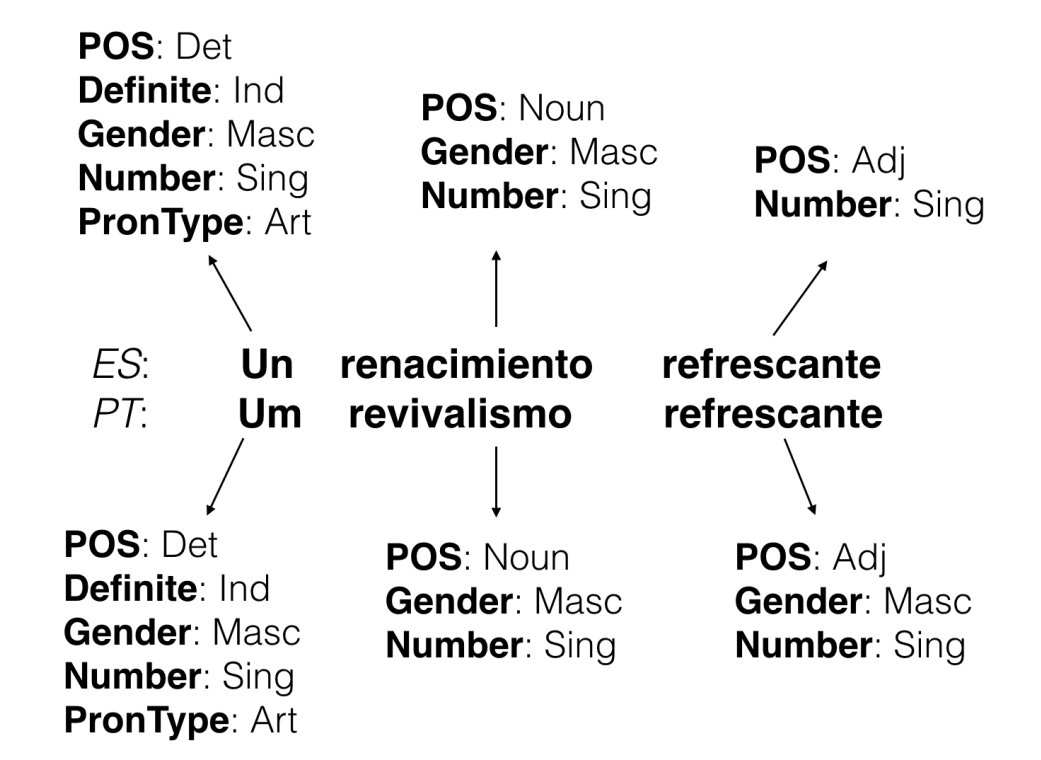
\includegraphics[width=0.8\textwidth]{morphy.png}
        % 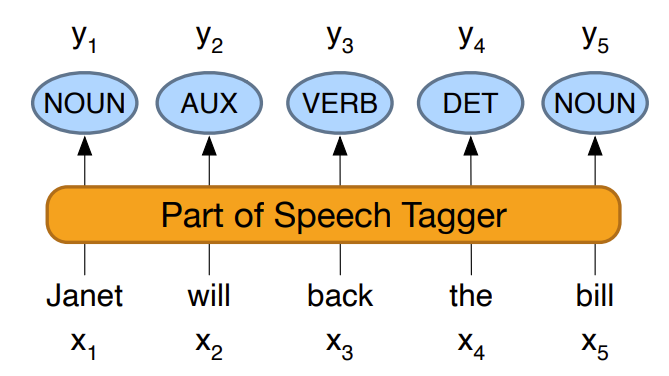
\includegraphics[width=0.40\textwidth]{pos.png}
        \caption{Tag morphologique d'une phrase portugaise et sa traduction en espagnol.}
    \end{figure}
\end{frame}

\begin{frame}{Le dataset}
    Nous avons utilisé le dataset Universal Dependencies 2.13.

    Le dataset en français contient :
    \begin{itemize}
        \item 47498 phrases
        \item 849476 mots
        \item 76048 mots uniques
    \end{itemize}

    On a recensé :
    \begin{itemize}
        \item 19 classes \textit{pos}.
        \item 28 classes \textit{morphy}, avec un nombre de possibilités entre 2 et 13
    \end{itemize}
\end{frame}

\begin{frame}{Les \textit{morphy}}
    \begin{figure}
        \centering
        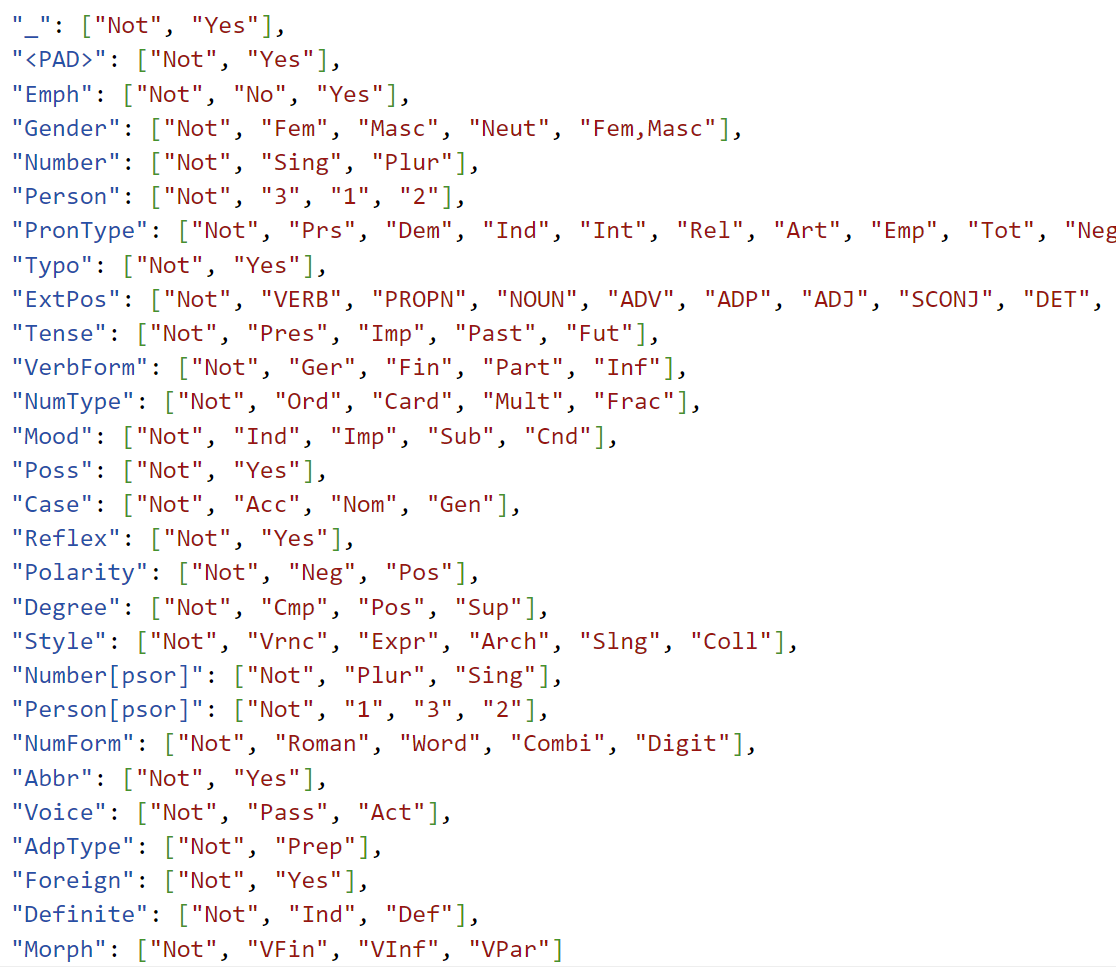
\includegraphics[width=0.8\textwidth]{all_morphy.png}
        % \caption{Ensemble de tous les \textit{morphy}}
    \end{figure}
\end{frame}

\begin{frame}{création de séquences}
    \begin{exampleblock}{Idée}
        On rajoute des caractères $\langle$PAD$\rangle$ pour compléter les phrases,
        on rajoute aussi un label qui correspond au pad.
    \end{exampleblock}

    \bigskip
    Si on fixe une longueur de séquence à 5, on va transformer la phrase :
    \begin{table}
        \centering
        \begin{tabular}{|c|c|c|}
            \hline
            \textbf{type} & \textbf{exemple} & \textbf{longueur} \\
            \hline
            phrase & Les poissons sont des animaux vertébrés . & 7 \\
            \hline
            Séquence & Les poissons sont des animaux & 5\\
             & vertébrés . $\langle$PAD$\rangle$ $\langle$PAD$\rangle$ $\langle$PAD$\rangle$ & 5\\
            \hline
        \end{tabular}
        \caption{Exemple de la création du séquences}
    \end{table}
\end{frame}

\begin{frame}{La gestion des mots inconnus}
    \begin{exampleblock}{Idée}
        Si le modèle rencontre un mot inconnus, il va le remplacer par le mot $\langle$UNK$\rangle$.
        Le modèle doit alors aussi apprendre ce mot lors de l'entraînement.
    \end{exampleblock}

    \begin{itemize}
        \item Avant l'entraînement, on fait un dropout des mots avec un taux d'oublie de $1\%$.
        \item On obtient un nombre de mots dans le vocabulaire de taille 67814 (contre 76048 dans le dataset).
        \item On a fixé la seed avant
    \end{itemize}
\end{frame}

\begin{frame}{Encodage des labels}
    Pour les \textit{pos} :
    \begin{itemize}
        \item On remplace le label par son indice dans la liste des labels.
    \end{itemize}
    Pour les \textit{morphy} :
    \begin{itemize}
        \item On remplace le label par une liste d'indice, où l'élément $i$ de la liste correspond à l'indice du $i$-ème type de morphy.
    \end{itemize}
    Exemple : \textit{Emph=No$\mid$Number=Sing$\mid$Person=1$\mid$PronType=Prs}

    [0, 0, 1, 0, 1, 2, 9, 0, 0, 0, 0, 0, 0, 0, 0, 0, 0, 0, 0, 0, 0, 0, 0, 0, 0, 0, 0, 0]

    \begin{exampleblock}{Shape}
        \begin{itemize}
            \item Entrée : $x$ de taille $B \times K$ contenant les indices des mots
            \item Sortie de \textit{pos}: $y_{pos}$ de taille $B \times K \times 19$
            \item Sortie de \textit{morphy}: $y_{morphy}$ de taille $B \times K \times 28 \times 13$
        \end{itemize}
    \end{exampleblock}
\end{frame}

\begin{frame}{Modèle \textit{GET\_POS}}
    \begin{figure}
        \centering
        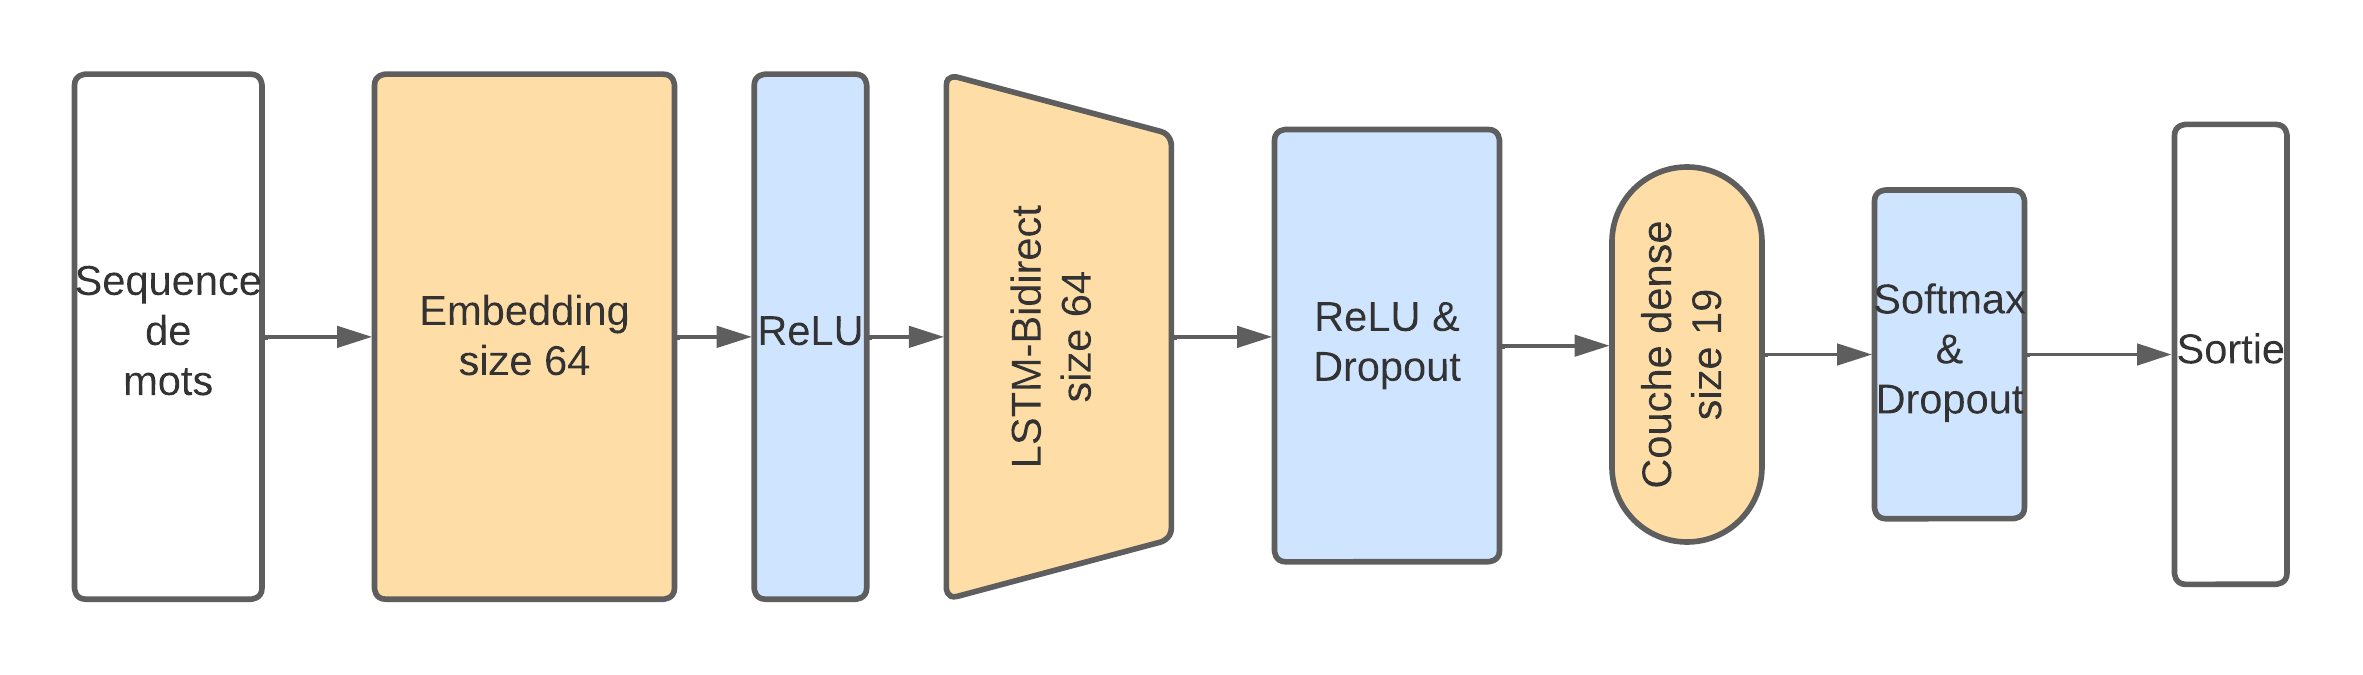
\includegraphics[width=\textwidth]{get_pos.png}
        \caption{Modèle \textit{GET\_POS}}
        \label{fig: model getpos}
    \end{figure} 
\end{frame}

\begin{frame}{Modèle \textit{SUPERTAG}}
    \begin{figure}
        \centering
        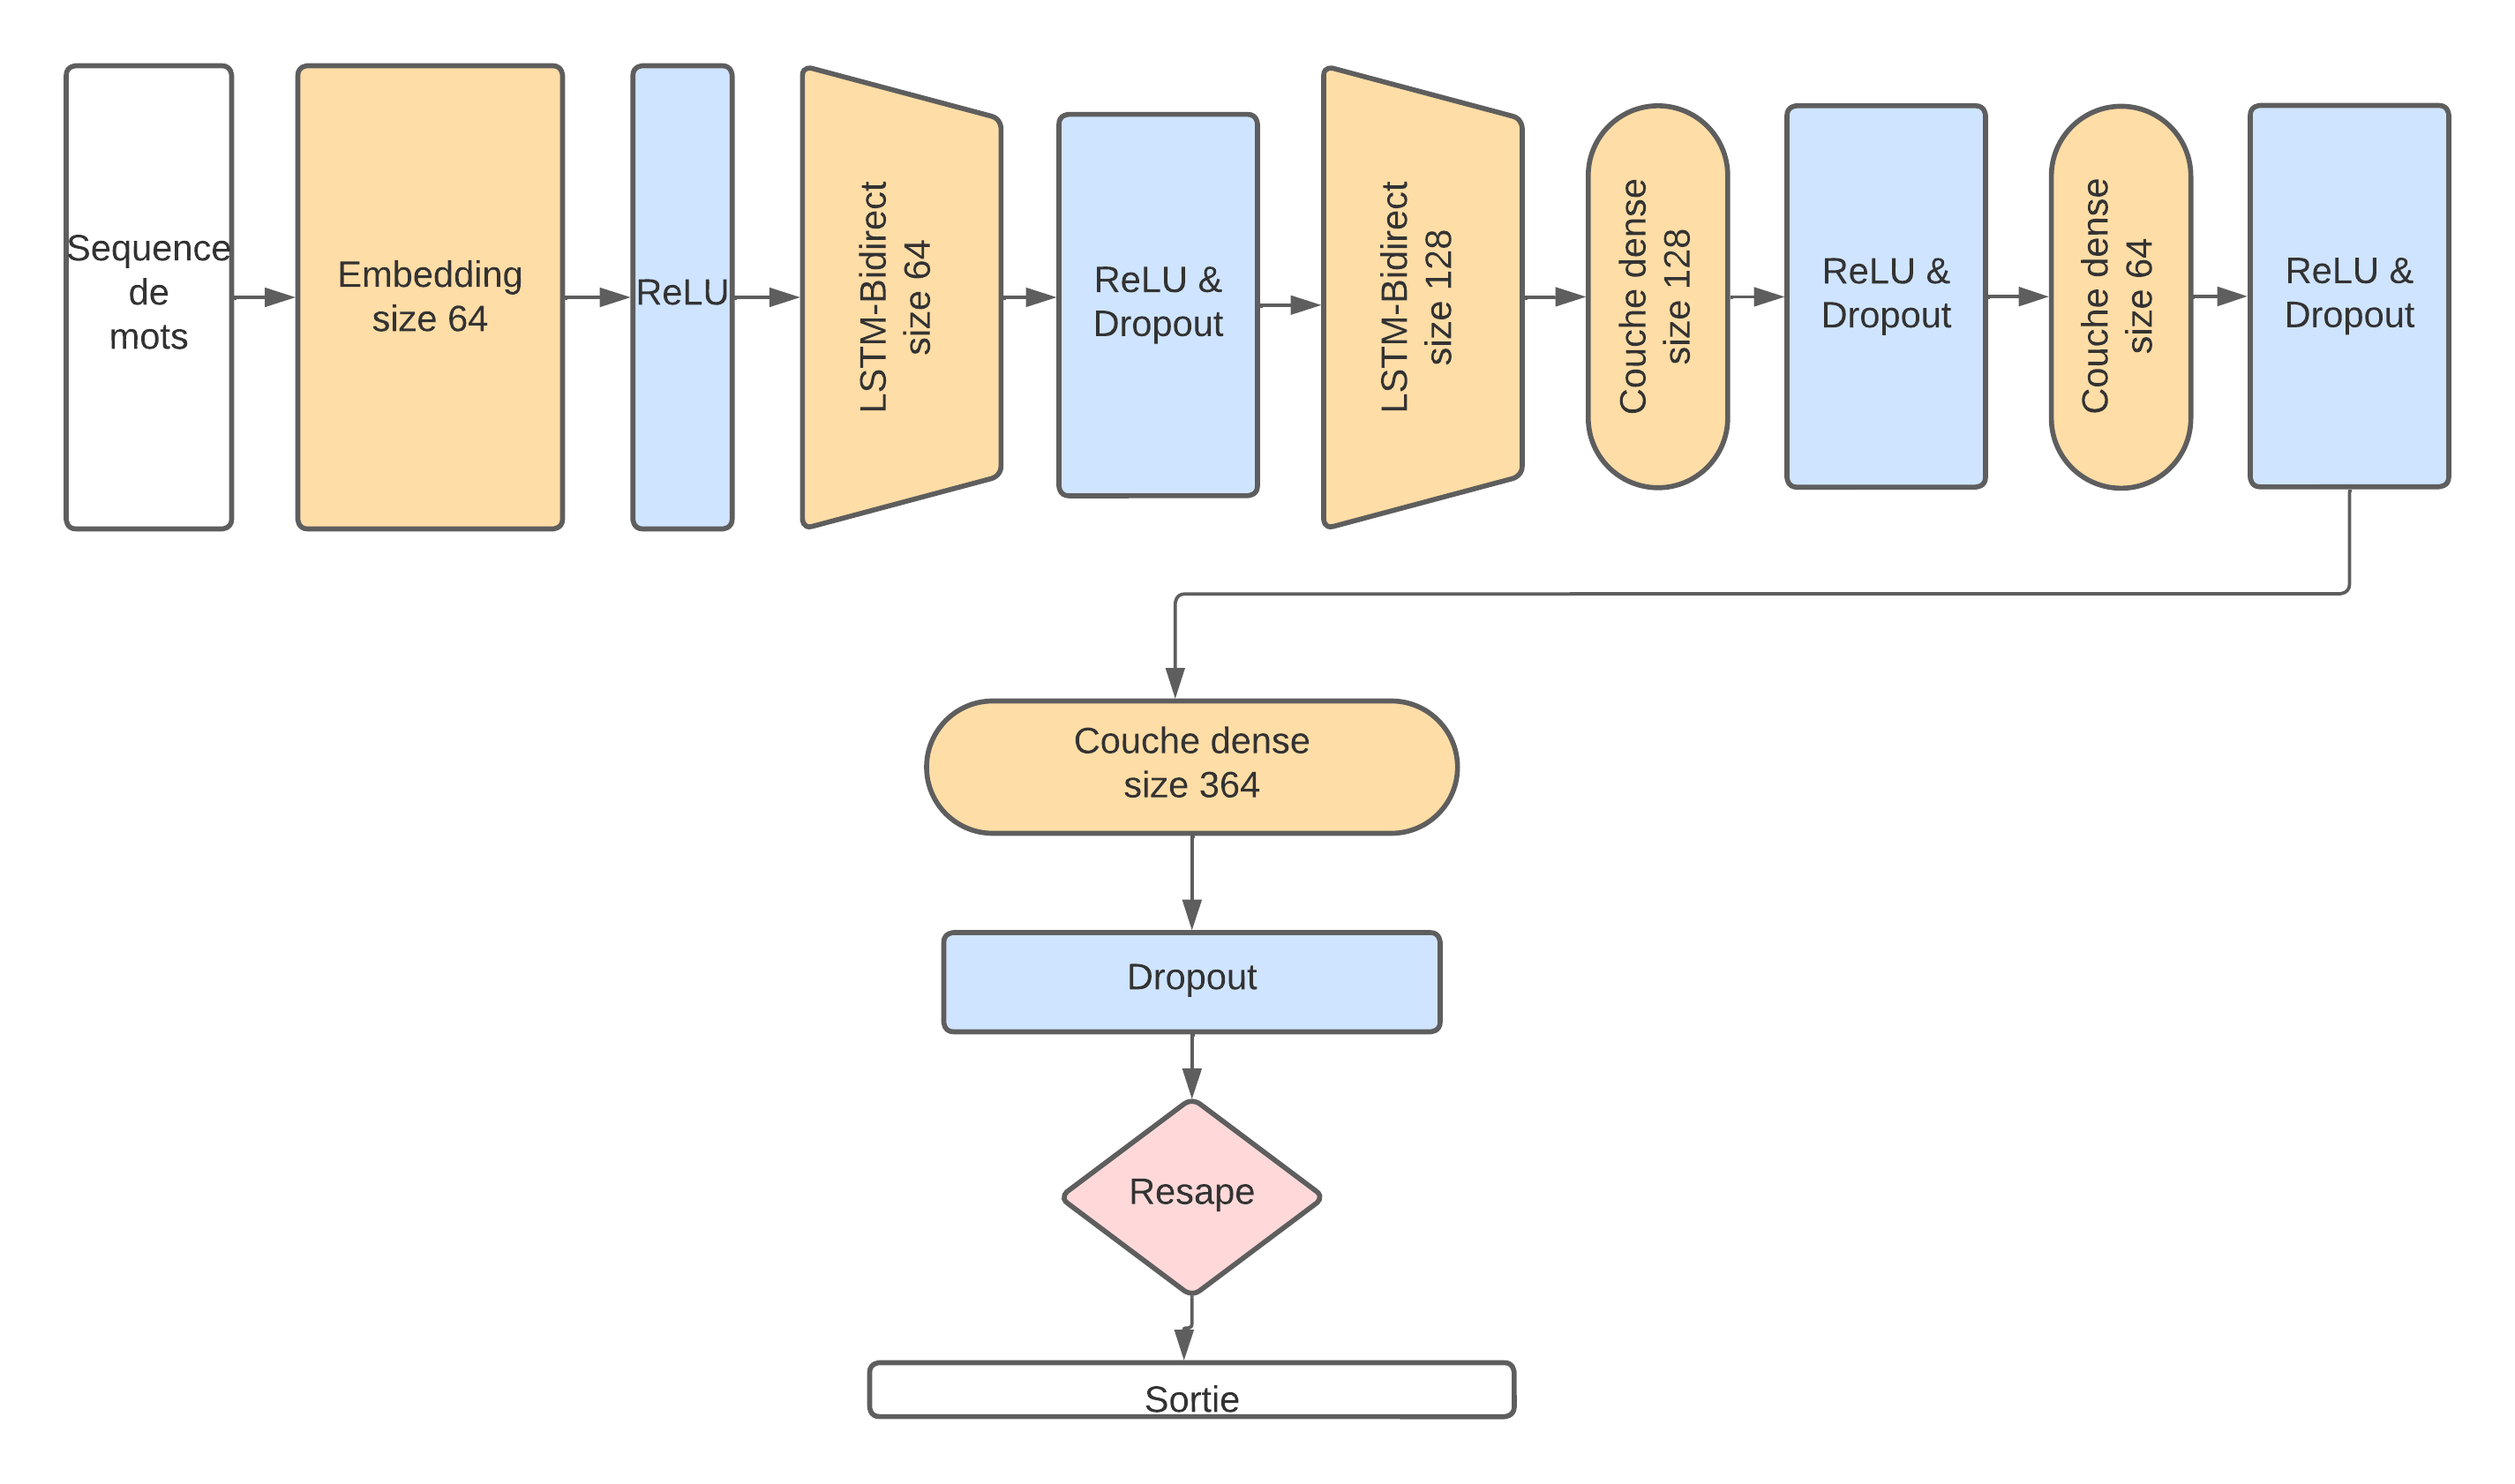
\includegraphics[width=\textwidth]{get_morphy_supertag.png}
        \caption{Modèle \textit{SUPERTAG}}
        \label{fig: model supertag}
    \end{figure}
\end{frame}

\begin{frame}{Modèle \textit{SEPARATE}}
    \begin{figure}
        \centering
        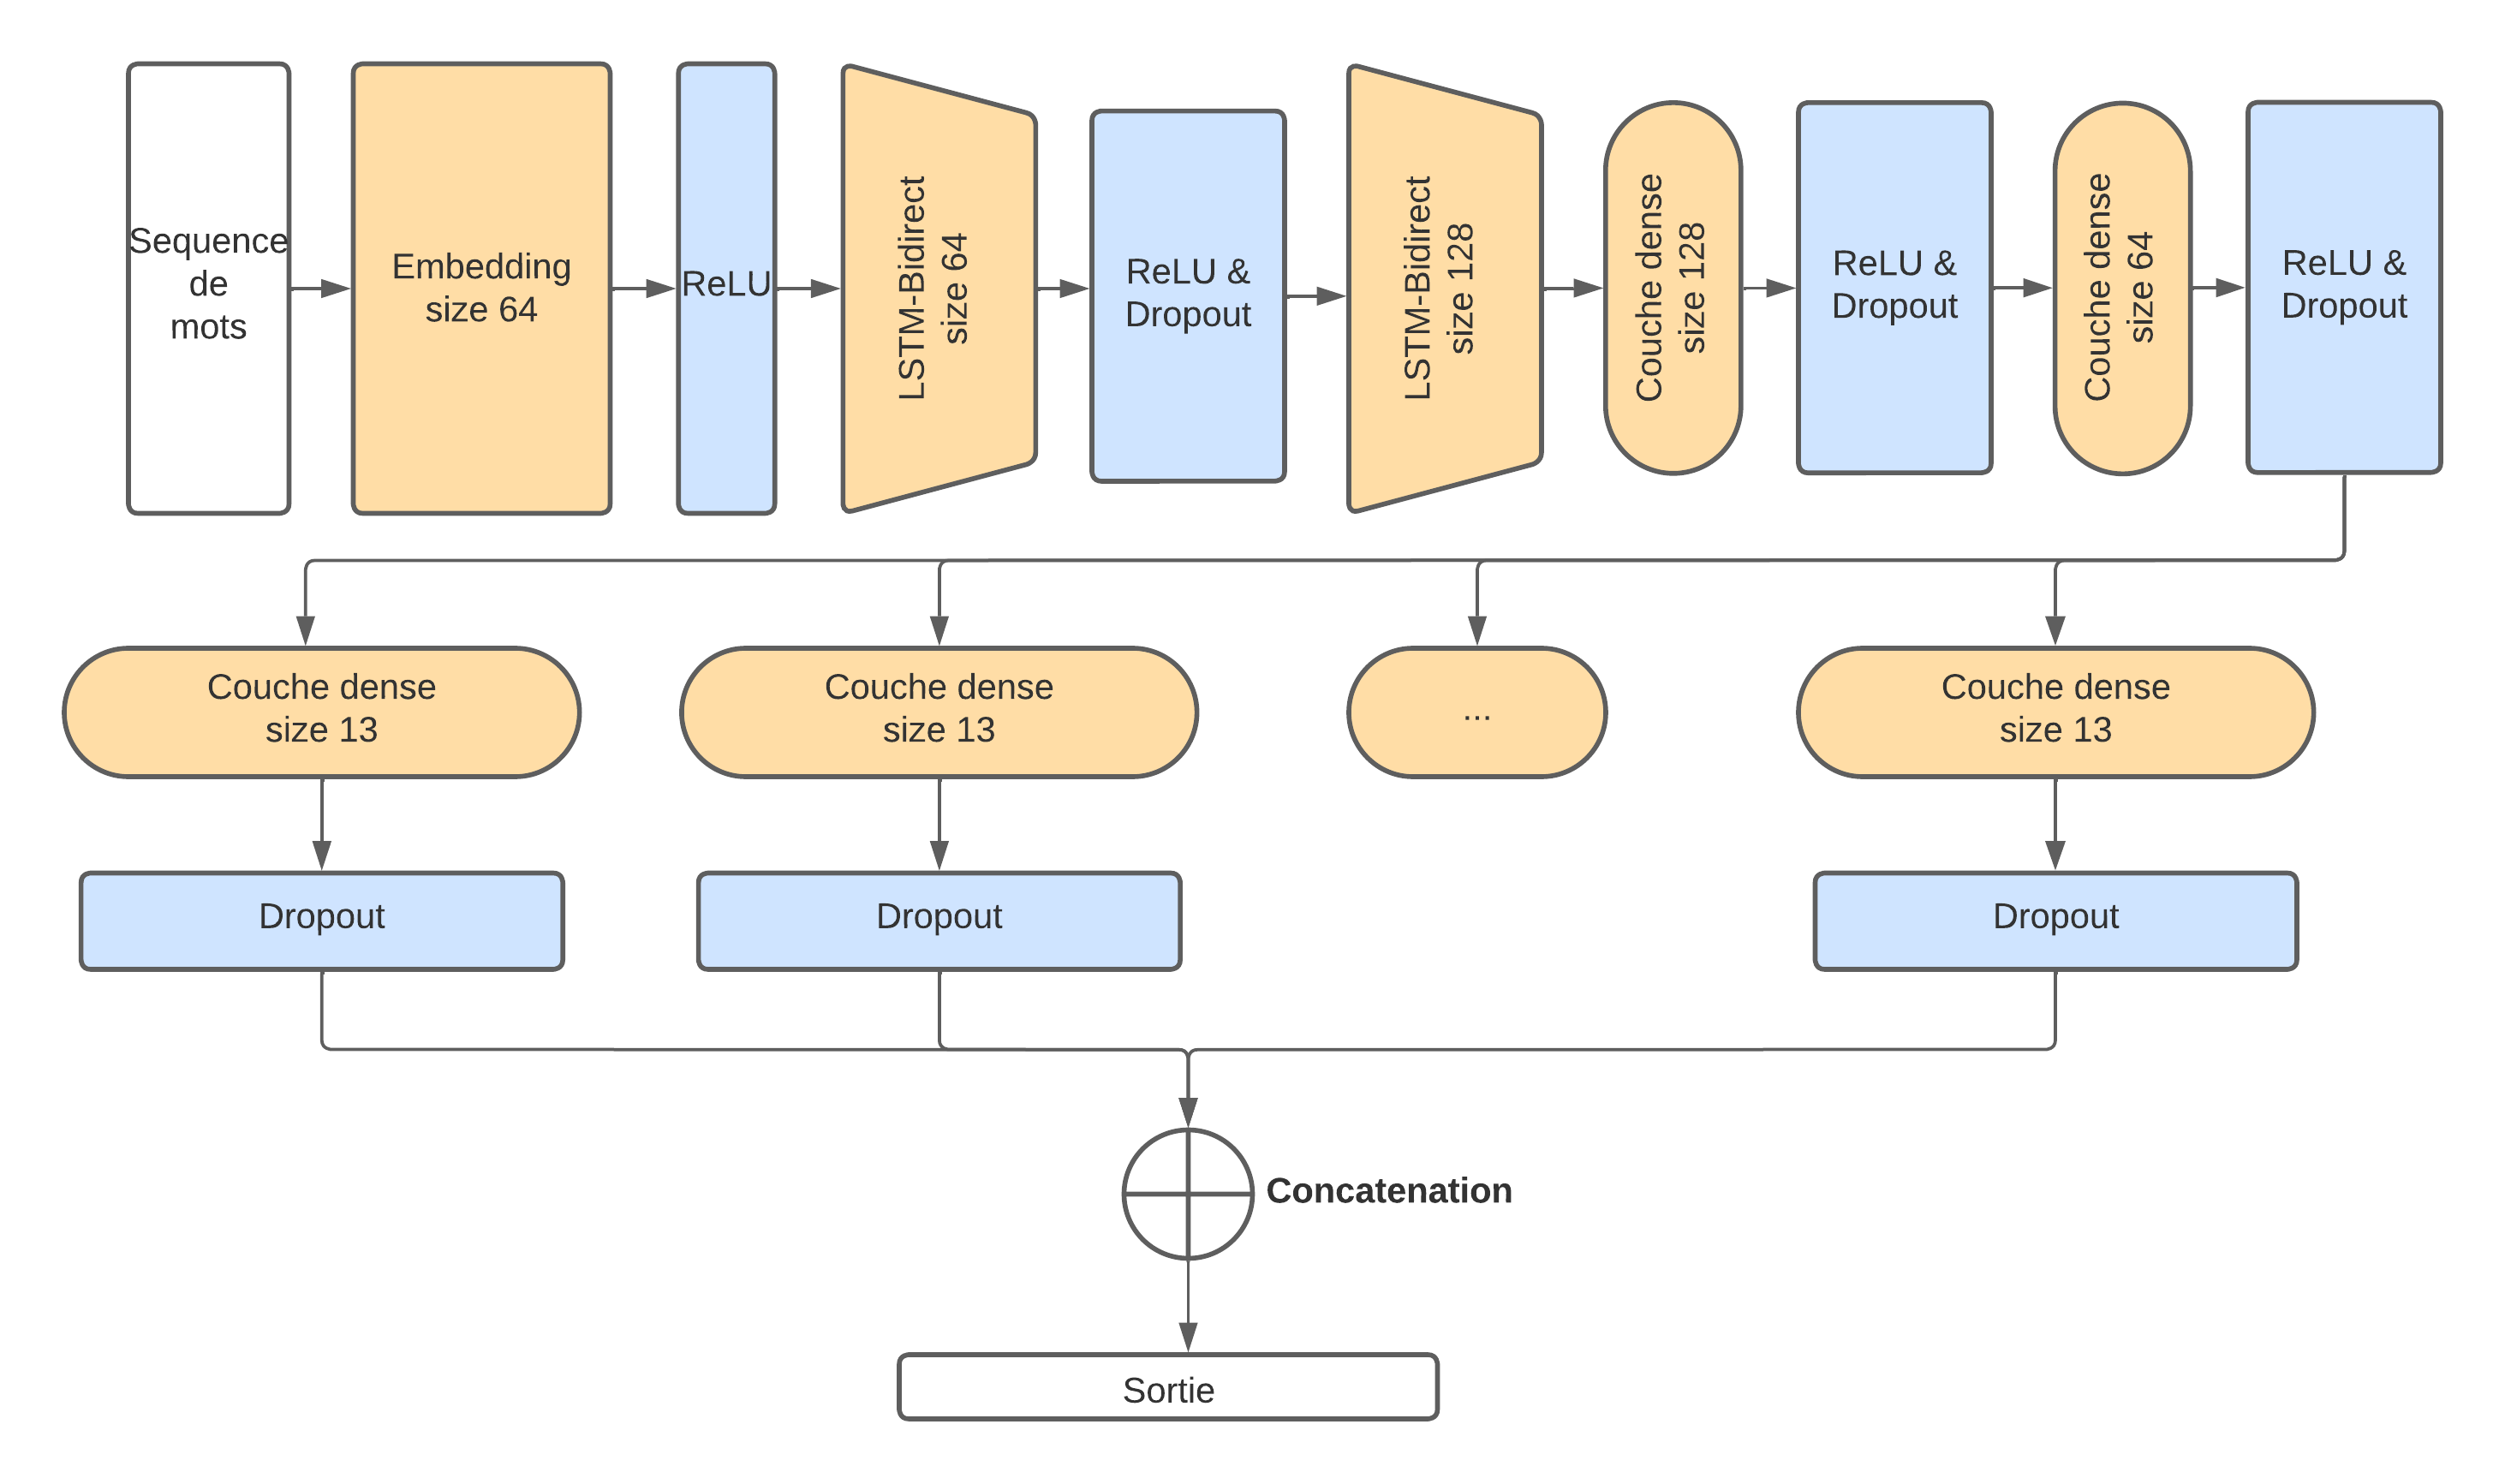
\includegraphics[width=\textwidth]{get_morphy_separate.png}
        \caption{Modèle \textit{SEPARATE}.}
        \label{fig: model separate}
    \end{figure}
\end{frame}

\begin{frame}{Modèle \textit{FUSION}}
    \begin{figure}[!ht]
        \centering
        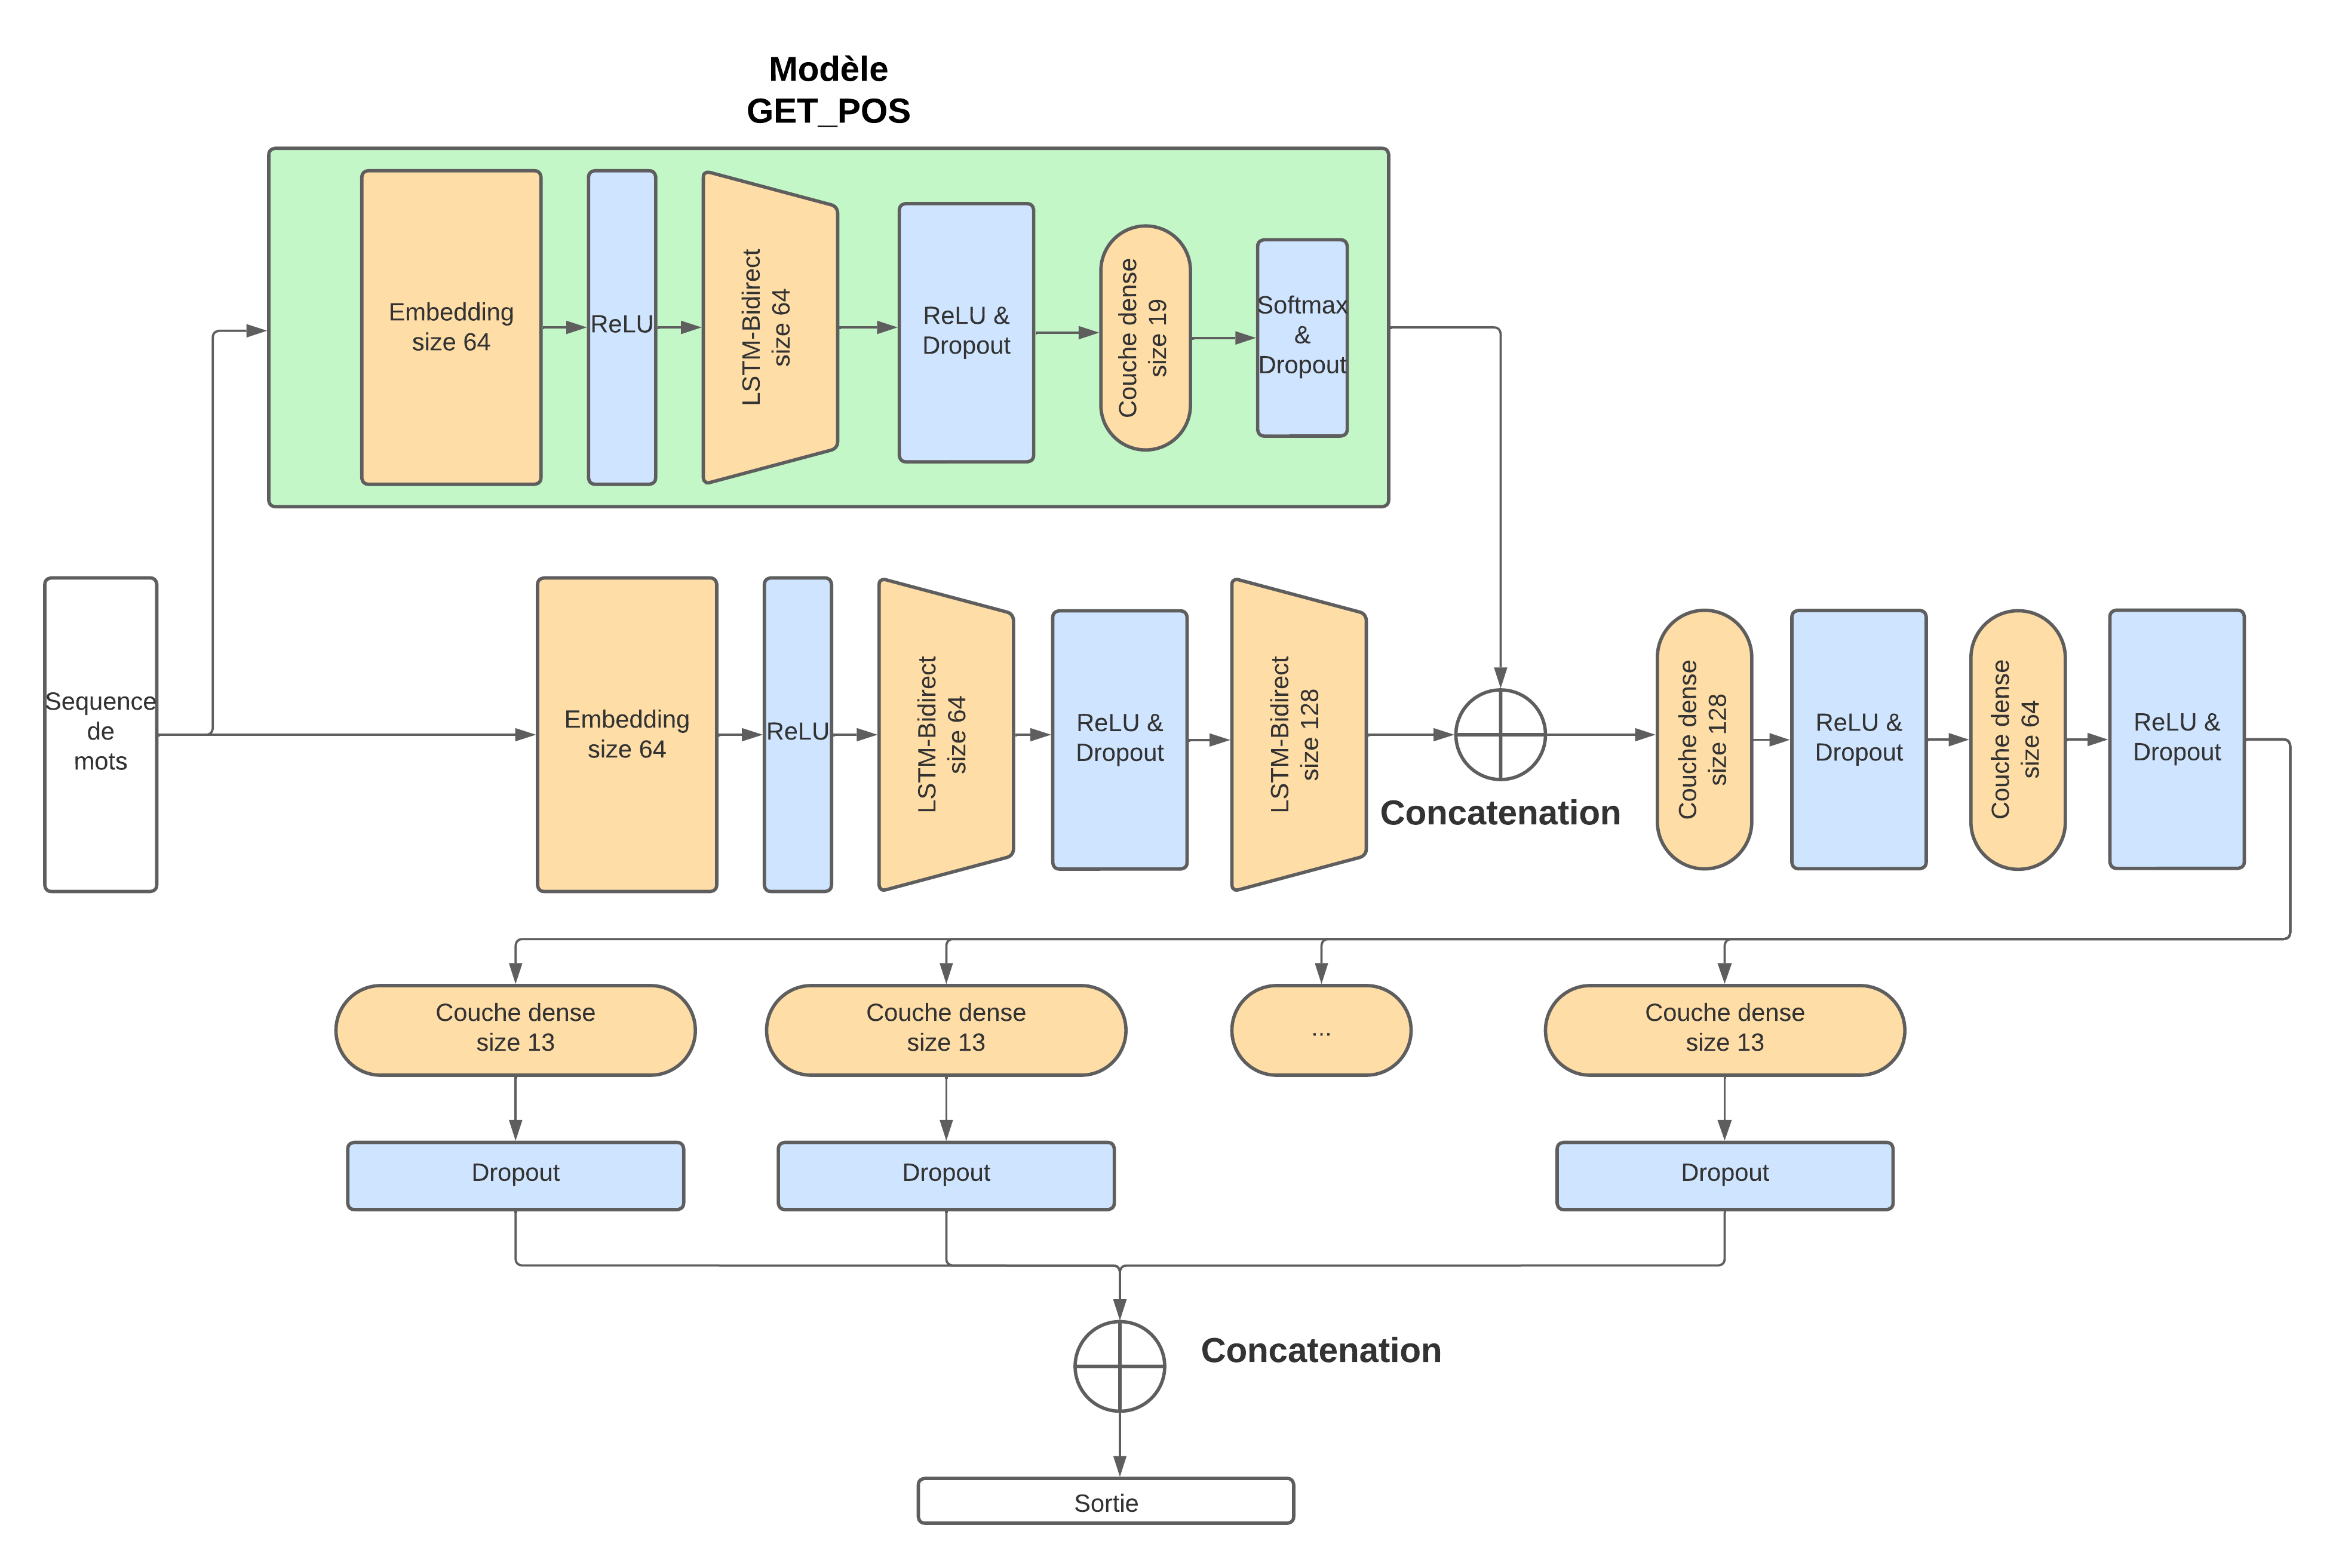
\includegraphics[width=0.9\textwidth]{get_morphy_fusion.png}
        \caption{Modèle \textit{FUSION}}
        \label{fig: model fusion}
    \end{figure}
\end{frame}

\begin{frame}{Loss et Métriques}
    Les loss :
    \begin{itemize}
        \item crossentropy pour le \textit{pos}
        \item moyenne de la crossentropy sur les 28 classes pour le \textit{morphy}
    \end{itemize}
    Les métriques :
    \begin{itemize}
        \item accuracy micro
        \item accuracy macro (pour le \textit{pos})
        \item allgood (pour le \textit{morphy})
    \end{itemize}
\end{frame}

\begin{frame}{Résultats : \textit{GET\_POS}}
    \begin{figure}
        \centering
        \begin{subfigure}{0.32\textwidth}
            \centering
            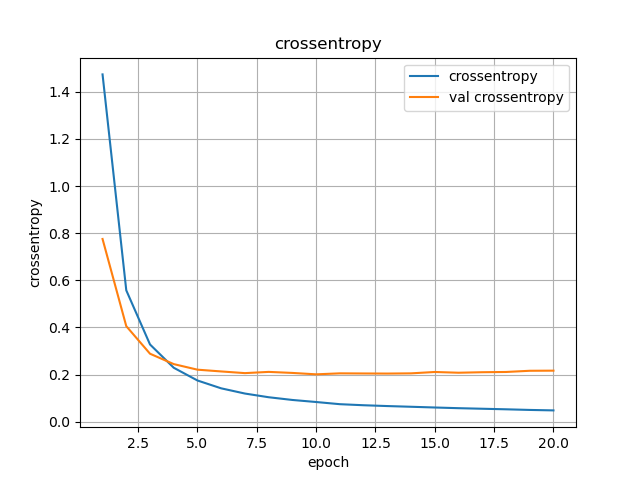
\includegraphics[width=\linewidth]{../logs/get_pos/crossentropy.png}
        \end{subfigure}
        \begin{subfigure}{0.32\textwidth}
            \centering
            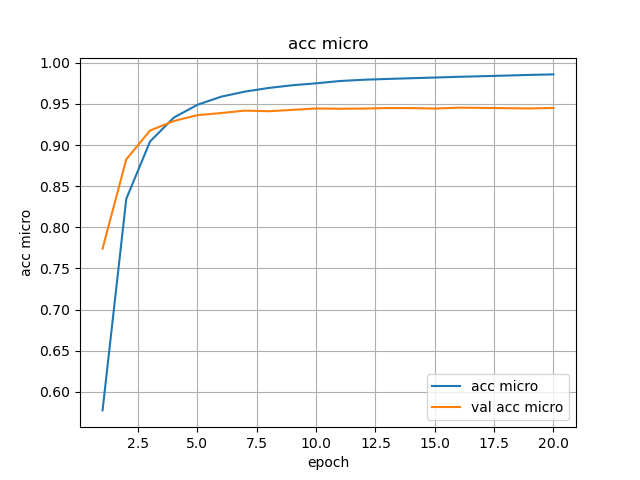
\includegraphics[width=\linewidth]{../logs/get_pos/acc micro.png}
        \end{subfigure}
        \begin{subfigure}{0.32\textwidth}
            \centering
            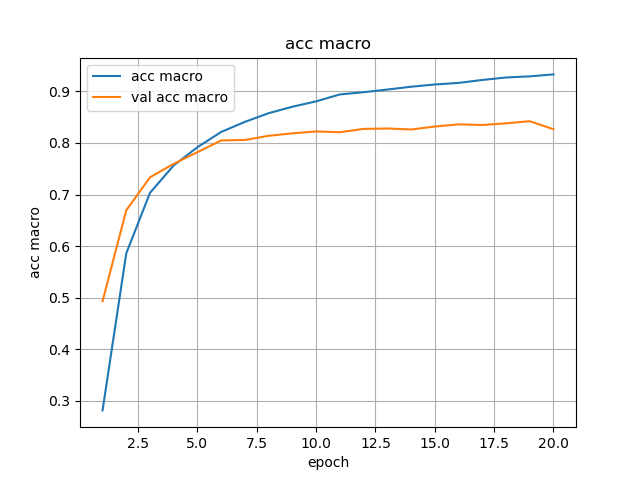
\includegraphics[width=\linewidth]{../logs/get_pos/acc macro.png}
        \end{subfigure}
        \caption{Entraînement du modèle \textit{GET\_POS}.}
    \end{figure}

    \begin{table}
        \centering
        \begin{tabular}{|c|c|c|c|}
            \hline
            Nom du modèle & crossentropy & accuracy micro & accuracy macro \\
            \hline
            \textit{GET\_POS} & 0.204 & 0.944 & 0.816\\
            \hline
        \end{tabular}
        \caption{Résultats du modèle \textit{GET\_POS} sur la base de données de teste.}
        \label{tab:test getpos}
    \end{table}
\end{frame}

\begin{frame}{Résultats des modèles \textit{SUPERTAG} et \textit{SEPARATE}}
    \begin{figure}
        \centering
        \begin{subfigure}{0.32\textwidth}
            \centering
            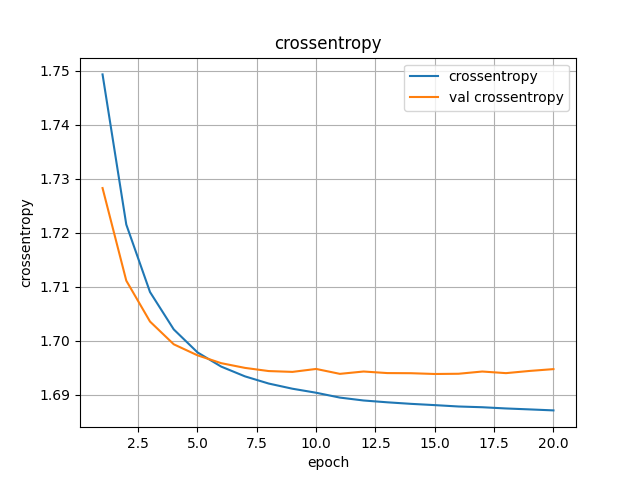
\includegraphics[width=\linewidth]{../logs/supertag/crossentropy.png}
        \end{subfigure}
        \begin{subfigure}{0.32\textwidth}
            \centering
            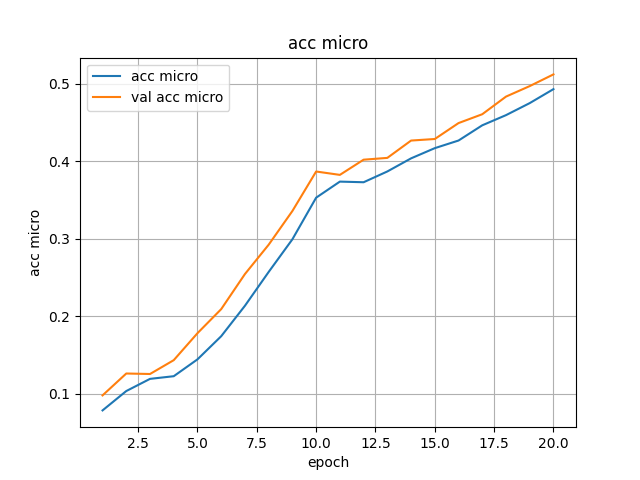
\includegraphics[width=\linewidth]{../logs/supertag/acc micro.png}
        \end{subfigure}
        \begin{subfigure}{0.32\textwidth}
            \centering
            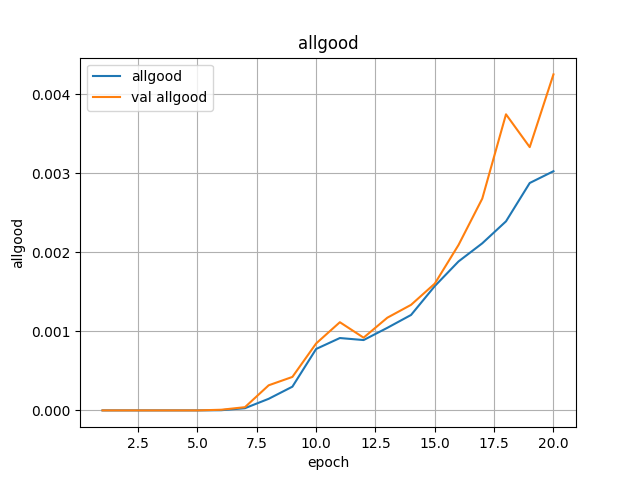
\includegraphics[width=\linewidth]{../logs/supertag/allgood.png}
        \end{subfigure}
        \caption{Entraînement du modèle \textit{SUPERTAG}.}
        \label{fig: results supertag}
    \end{figure}
    \begin{figure}
        \centering
        \begin{subfigure}{0.32\textwidth}
            \centering
            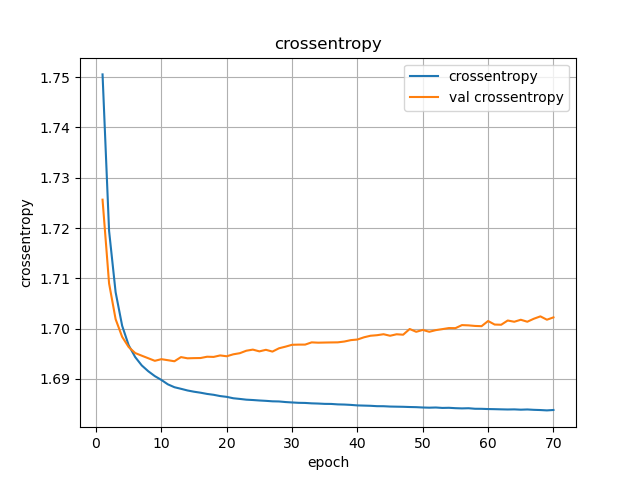
\includegraphics[width=\linewidth]{../logs/separate/crossentropy.png}
        \end{subfigure}
        \begin{subfigure}{0.32\textwidth}
            \centering
            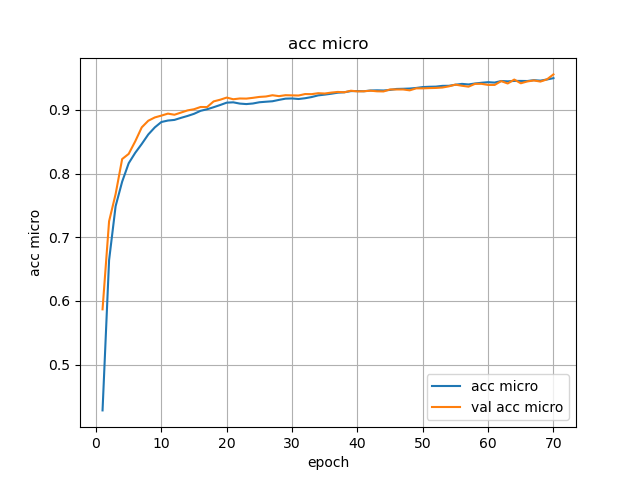
\includegraphics[width=\linewidth]{../logs/separate/acc micro.png}
        \end{subfigure}
        \begin{subfigure}{0.32\textwidth}
            \centering
            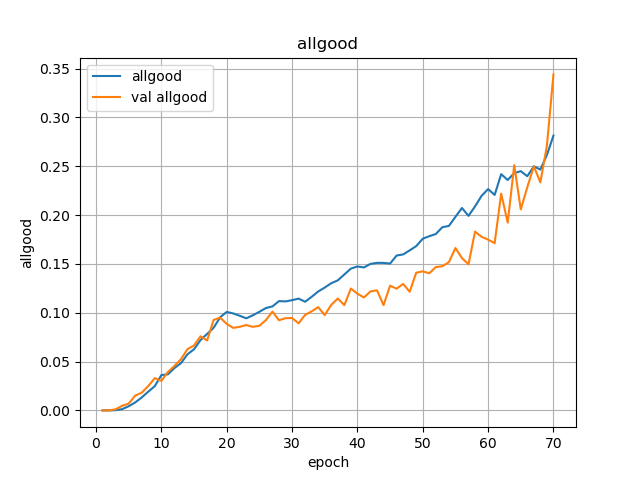
\includegraphics[width=\linewidth]{../logs/separate/allgood.png}
        \end{subfigure}
        \caption{Entraînement du modèle \textit{SEPARATE}.}
        \label{fig: results separate}
    \end{figure}
\end{frame}

\begin{frame}{Résultats du modèle \textit{FUSION} et résultats de teste}
    \begin{figure}
        \centering
        \begin{subfigure}{0.32\textwidth}
            \centering
            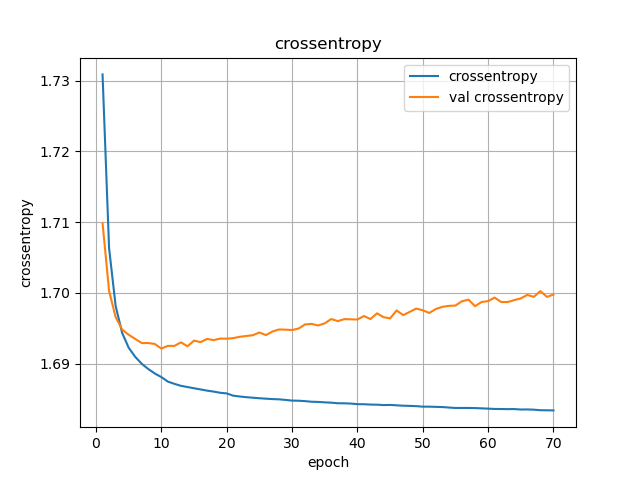
\includegraphics[width=\linewidth]{../logs/fusion/crossentropy.png}
        \end{subfigure}
        \begin{subfigure}{0.32\textwidth}
            \centering
            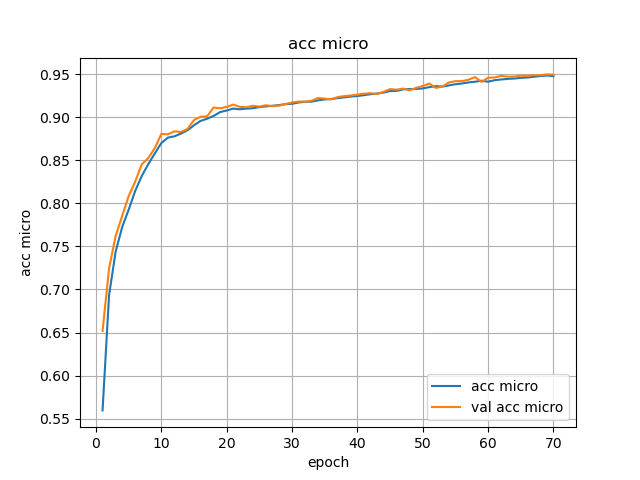
\includegraphics[width=\linewidth]{../logs/fusion/acc micro.png}
        \end{subfigure}
        \begin{subfigure}{0.32\textwidth}
            \centering
            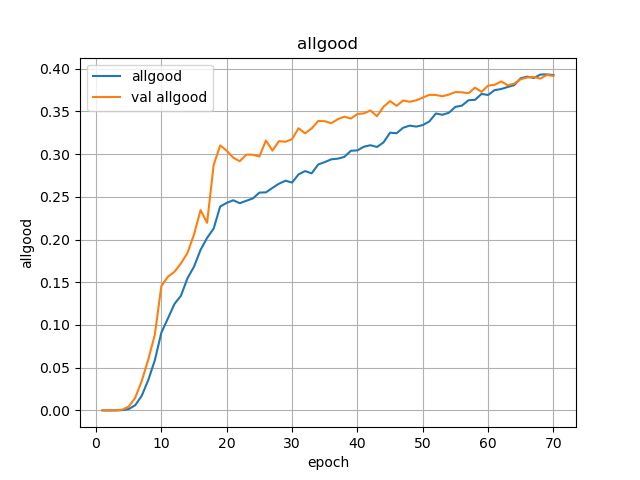
\includegraphics[width=\linewidth]{../logs/fusion/allgood.png}
        \end{subfigure}
        \caption{Entraînement du modèle \textit{FUSION}.}
        \label{fig: results fusion}
    \end{figure}

    \begin{table}
        \centering
        \begin{tabular}{|c|c|c|c|}
            \hline
             Nom du modèle & crossentropy & accuracy micro & all good\\
             \hline
             \textit{BASELINE}& - & 0.980 & 0.791 \\
             \hline
             \textit{SUPERTAG}& 1.700 & 0.436 & 0.002\\
             \hline
             \textit{SEPARATE}& 1.70 & 0.893 & 0.046\\
             \hline
             \textit{FUSION}& 1.698 & 0.884 & 0.154 \\
             \hline
        \end{tabular}
        \caption{Résultats de test sur la prédiction des \textit{morphy}}
        \label{tab: test morphy}
    \end{table}
\end{frame}

\begin{frame}{Inférences}
    Inférences sur la phrase : \textit{Les bananes sont jaunes et mûrs.} \\
    un mot inconnu : \textit{mûrs}
    \begin{table}
        \centering
        \begin{tabular}{|c|c|}
            \hline
            \textbf{modèle} & \textbf{inférences} \\
            \hline
            \textit{BASELINE} & Gender=Fem$\mid$Number=Plur \\
            \hline
            \textit{SUPERTAG} & NumForm=Roman$\mid$Abbr=Yes$\mid$Morph=VInf\\
            \hline
            \textit{SEPARATE} & Gender=Neut$\mid$Number=Plur$\mid$VerbForm=Ger\\
             & Degree=Pos$\mid$Abbr=Yes\\
            \hline
            \textit{FUSION} & Gender=Fem,Masc$\mid$Number=Plur$\mid$PronType=Tot\\
             & NumType=Mult$\mid$Case=Nom$\mid$NumForm=Combi\\
            \hline
        \end{tabular}
        \caption{Inférences du mot \textit{bananes}}
    \end{table}
\end{frame}

\begin{frame}{Inférences}
    \begin{table}
        \centering
        \begin{tabular}{|c|c|}
            \hline
            \textbf{modèle} & \textbf{inférences} \\
            \hline
            \textit{BASELINE} & $\langle$PAD$\rangle$=Yes \\
            \hline
            \textit{SUPERTAG} & PronType=Emp$\mid$Style=Coll\\
            \hline
            \textit{SEPARATE} & $\langle$PAD$\rangle$=Yes$\mid$PronType=Int,Rel$\mid$Case=Nom\\
             & Degree=Sup$\mid$NumForm=Combi\\
            \hline
            \textit{FUSION} & $\langle$PAD$\rangle$=Yes$\mid$Gender=Neut$\mid$PronType=Int,Rel\\
             & NumType=Mult$\mid$Degree=Sup$\mid$Style=Slng\\
             & NumForm=Combi\\
            \hline
        \end{tabular}
        \caption{Inférences du dernier$\langle$PAD$\rangle$.}
    \end{table}
\end{frame}

\begin{frame}{Nos difficultés rencontrées}
    \begin{itemize}
        \item Trouver la bonne loss pour les \textit{morphy}. Car avant, on avait seulement 
            la crossentropy et 0.02\% d'accuracy.
        \item Dans le modèle \textit{SEPARATE}, on a l'ensemble des dernières couches 
            Dense dans une liste. Et donc le \textit{model.parameters()} ne donnent pas les 
            paramètres de ces couches.
        \item Avant, on n'avait pas ajouté les $-\infty$ dans le modèle \textit{SEPARATE},
            donc on avait de moins bonnes performances
    \end{itemize}
\end{frame}

\begin{frame}{Les pistes d'améliorations}
    \begin{itemize}
        \item Changer la façon dont on crée les séquences.
        \item Ne pas prendre en comte les $\langle$PAD$\rangle$ dans la loss et les métriques.
        \item Changer la façon de mettre des mots inconnus. Car là, les mots inconnus 
            ne changent pas sur les epochs.
        \item comparer les résultats en fonction de la taille des séquences
        \item Mettre une couche Dense après les couches separate.
        \item Remplacer les modules LSTM par des Transformers.
    \end{itemize}
\end{frame}





\end{document}

